\section{Leis dos Cossenos e dos Senos}

\begin{theorem}[Lei dos Cossenos]
    Seja $ABC$ um triângulo com $a = \seg {BC}$, $b = \seg {AC}$ e $c = \seg
{AB}$. Então:
$$b^2 = a^2 + c^2 - 2 ac \cdot \cos \widehat B.$$
\end{theorem}

\begin{proof}
    Considere, na prova, o triângulo retângulo mostrado na Imagem~\ref{img:prova-lei-dos-cossenos}. % TODO: update \ref.
    %
    \begin{figure}[H]
        \centering
        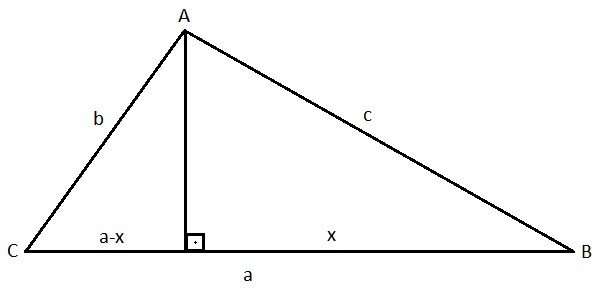
\includegraphics[scale=0.50]{\imgdirfromsection/fig-c10-theo1516-paint.jpg}
        \caption{Triângulo retângulo qualquer.}
        \label{img:prova-lei-dos-cossenos}
    \end{figure}
    %
    Note que $\cos \widehat B = \frac x c$, o que implica que:
    %
    \begin{equation}
    \label{eq:prova-lei-cossenos-1}
        x = c \cos \widehat B
    \end{equation}
    %
    Agora, usando o Teorema de Pitágoras no triângulo $\triangle APB$, temos que:
    %
    \begin{equation}
    \label{eq:prova-lei-cossenos-2}
        c^2 = x^2 + h^2
    \end{equation}
    %
    Aplicando o mesmo teorema no triângulo $\triangle APC$, obtemos:
    %
    \begin{equation}
    \label{eq:prova-lei-cossenos-3}
        b^2 = \prn{a-x}^2+h^2 = a^2 - 2ax+x^2 + h^2
    \end{equation}
    %
    De \ref{eq:prova-lei-cossenos-2} e \ref{eq:prova-lei-cossenos-3}, temos que:
    %
    \begin{align*}
        b^2 - c^2 = a^2 - 2ax + x^2 + h^2    -(x^2 + h^2) \stackrel{\ref{eq:prova-lei-cossenos-1}}{\iff} b^2 = a^2 + c^2 -2ac \cdot \cos \widehat B
    \end{align*}
\end{proof}

\begin{remark}
    A Lei dos Cossenos é uma generalização do Teorema de Pitágoras. Note
que, se $\widehat B$ é um ângulo reto, então $\cos \widehat B = 0$ e
$b$ será a hipotenusa do triângulo.
\end{remark}

\begin{theorem}[Lei dos Senos]
    Seja $ABC$ um triângulo com $a = \seg {BC}$, $b = \seg {AC}$ e $c = \seg
{AB}$. Então:
$$\frac a {\sen \widehat A} = \frac b {\sen \widehat B} = \frac c {\sen \widehat C}$$
\end{theorem}

\begin{proof}
    Consideremos, novamente, o triângulo retângulo da Imagem . %TODO: update ref
    Temos que:
    %
    \begin{equation}
    \label{eq:prova-lei-senos-1}
        \sen \widehat B = \frac h c \iff h = c \cdot \sen \widehat B
    \end{equation}
    %
    \begin{equation}
    \label{eq:prova-lei-senos-2}
        \sen \widehat C = \frac h b \iff h = b \cdot \sen \widehat C
    \end{equation}
    %
    De \ref{eq:prova-lei-senos-1} e \ref{eq:prova-lei-senos-2}, temos que $c \sen \widehat B = b \sen \widehat C$,
    o que implica que $$\frac b {\sen \widehat B} = \frac c {\sen \widehat C}.$$ Analogamente, 
    baixando a altura relativa ao vértice $B$, teremos: $$ \frac c {\sen \widehat C} = \frac a {\sen \widehat A}.$$
    Portanto, $$\frac a {\sen \widehat A} = \frac b {\sen \widehat B} = \frac c {\sen \widehat C}.$$
\end{proof}

As leis dos cossenos e dos senos permitem obter os seis elementos de
um triângulo quando são dados três deles, desde que um seja lado,
conforme os casos clássicos de congruência de triângulos.

\begin{onlineact}
    \khan{https://pt.khanacademy.org/math/trigonometry/trig-with-general-triangles/solving-general-triangles/e/law-of-sines-and-cosines-word-problems}
    {Problemas com Triângulos Gerais}.
\end{onlineact}